\label{eigentrust_section}
	\begin{figure}[H]
		\centering
		\begin{tikzpicture}[
		% This will show the frame around the figure
		show background rectangle]
		
		% Place first 6 items
		\node[module] (recommender) at (0,2) {Recommender};
		\node[module] (filterer) at (0,-1) {Filterer};
		
		
		\node (fit) at (0,0.5) [draw,thick,minimum width=3.5cm,minimum height=4cm] {};
		
		\node (db) at (6,2) [draw,thick,minimum width=2.5cm,minimum height=1cm] {Neo4j Db};
		
		
		%arrow between boxes
		\draw[<-,dashed] (db)-- node[above] {recommended} node[below] {products} ++ (recommender);
		
		\draw[->,dashed, sloped] (db)-- node[above] {transactions} node[below] {eigentrusts} ++ (filterer);
		
		\draw[<-] (recommender)--(filterer);
		
		\end{tikzpicture}
		\caption{Recommender Structure}
		\label{fig:eigentrust_structure}
	\end{figure}
	\subsubsection{About Eigentrust} \label{about_eigentrust}
	Eigentrust\cite{Eigentrust} is a reputation calculation algorithm mainly designed for peer-to-peer networks. In our case, Eigentrust represents how strongly connected the customers are to their communities. Eigentrust values calculated by the eigentrust module provided by TACoRec\cite{Tacorec} and stored in Neo4j database as a property of the relationship between a customer and his/her community. 
	\subparagraph{Problem encountered with Eigentrust:}
	Especially for the customers connected to communities with small size and low densities, eigentrust values stored in the database are either very small or equal to zero (check Figure \ref{fig:eigentrust_distribution_figure}). Most of the customers with zero eigentrust values are eliminated after filtering the network from customers with a small number of products. Unfortunately, eigentrust values ​​are still quite small.
\begin{figure}[h]
	\centering
	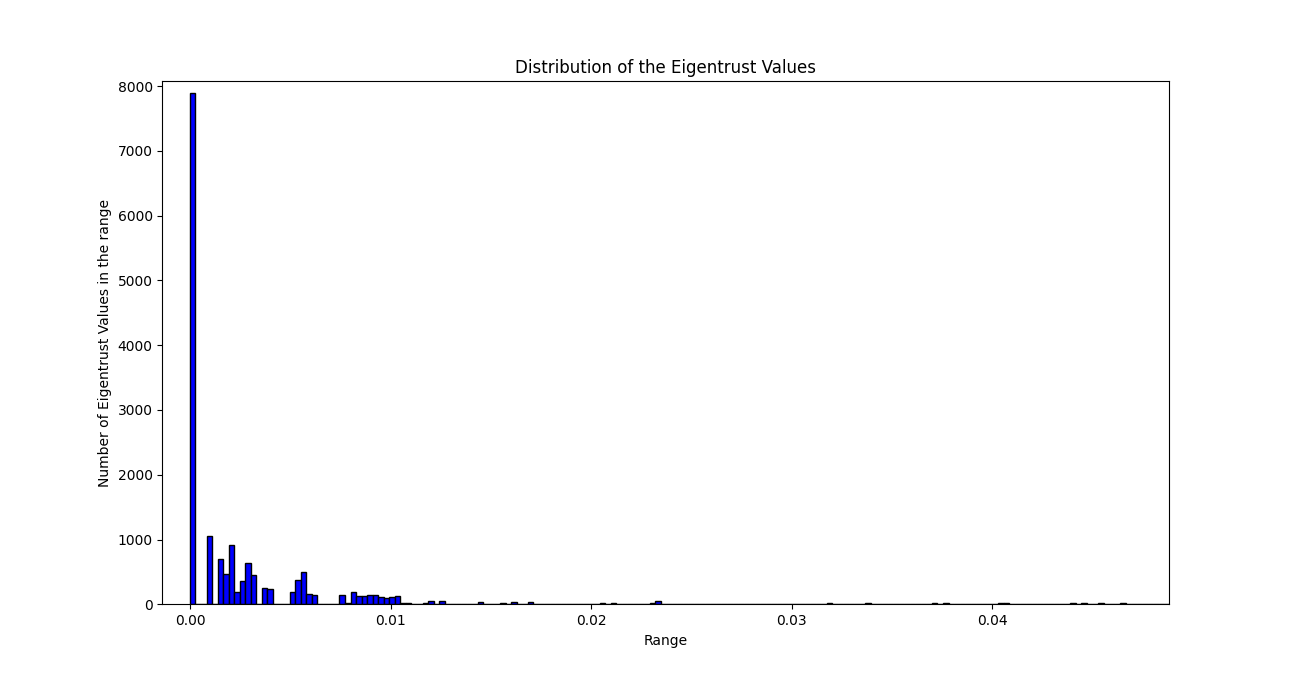
\includegraphics[scale=0.42]{eigentrust_distribution_detailed}
	\caption{Distribution of the Eigentrust Values. As can be seen nearly 8000 of the customers have zero eigentrust value.}
	\label{fig:eigentrust_distribution_figure}
\end{figure}
	\subsubsection{Filterer Module} 

	\subsubsection{Recommender Module} Recommender Module is basically responsible from reading/writing. The module has two tasks:
	\begin{enumerate}
		\item Getting transaction list which contains customer id product id pairs from the Neo4j database using neo4j driver and sending the list to the Filterer module as parameter.
		\item Getting the recommendation list which contains ids of the customers and corresponding recommended products from the Filterer module and writing these recommendations to Neo4j database as a relationship between the customer and the recommended product using neo4j driver.
	\end{enumerate}